\documentclass[12pt, twoside]{article}
\usepackage[francais]{babel}
\usepackage[T1]{fontenc}
\usepackage[latin1]{inputenc}
\usepackage[left=7mm, right=7mm, top=5mm, bottom=3mm]{geometry}
\usepackage{float}
\usepackage{graphicx}
\usepackage{array}
\usepackage{multirow}
\usepackage{amsmath,amssymb,mathrsfs}
\usepackage{soul}
\usepackage{textcomp}
\usepackage{eurosym}
 \usepackage{variations}
\usepackage{tabvar}


\pagestyle{empty}

\begin{document}


\section*{\center{Devoir maison 7}}


\medskip





\fbox{

\begin{minipage}{18cm}
\textit{Devoir � rendre sur feuille grand format pour le
\textbf{lundi 17 mai 2010}. Pr�sentation: 1 point.}
\end{minipage}
}

\bigskip



\ul{Exercice 1}: (\textit{5 points})

\begin{enumerate}
  \item Tracer un triangle FGH tel que: GF=5,2cm, $\widehat{HGF}=41$� et
  $\widehat{HFG}=63$�.
  \item Construire les m�diatrices ($d_1$) et ($d_2$) des c�t�s [HF] et [HG] de
  ce triangle. Ces deux droites se coupent en un point I.
  \item Tracer la m�diatrice du c�t� [GF]. V�rifier qu'elle passe aussi par I.
  \item Tracer le cercle circonscrit au triangle FGH.  
\end{enumerate}

\medskip




\ul{Exercice 2}: (\textit{3 points}) Calculer le p�rim�tre et l'aire des
triangles suivants:

\begin{center}
\begin{tabular}{cc}
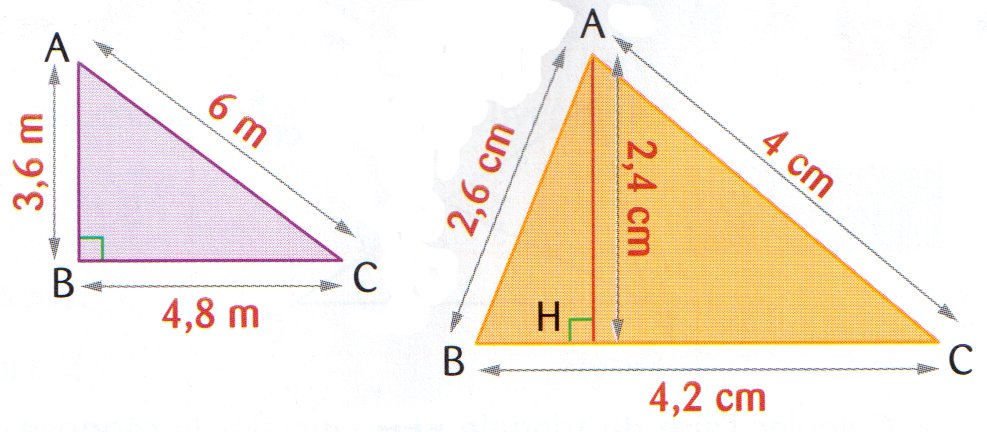
\includegraphics[width=6cm]{images/ex2-1.jpg} &
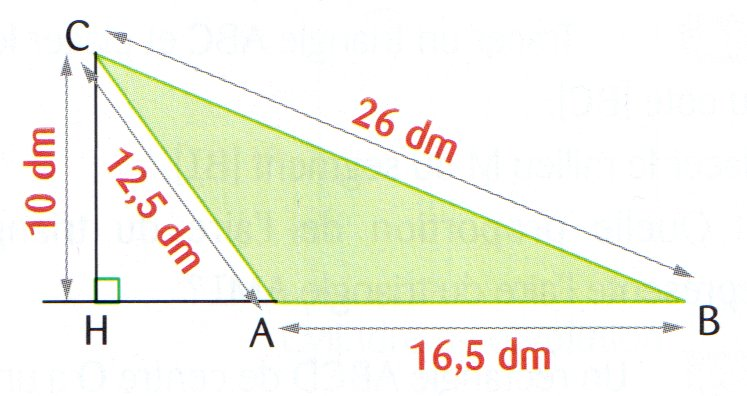
\includegraphics[width=5cm]{images/ex2-2.jpg} \\
\end{tabular}

\end{center}
 
 
\medskip



\begin{tabular}{ccc}
\begin{minipage}{7cm}
\ul{Exercice 3}: (\textit{3,5 points})

\enskip

Le quadrilat�re TRAP est un trap�ze. TRHK est un carr� de 4cm de c�t�. HA=5cm
et PK=3cm. Calculer l'aire du trap�ze TRAP.

\begin{center}
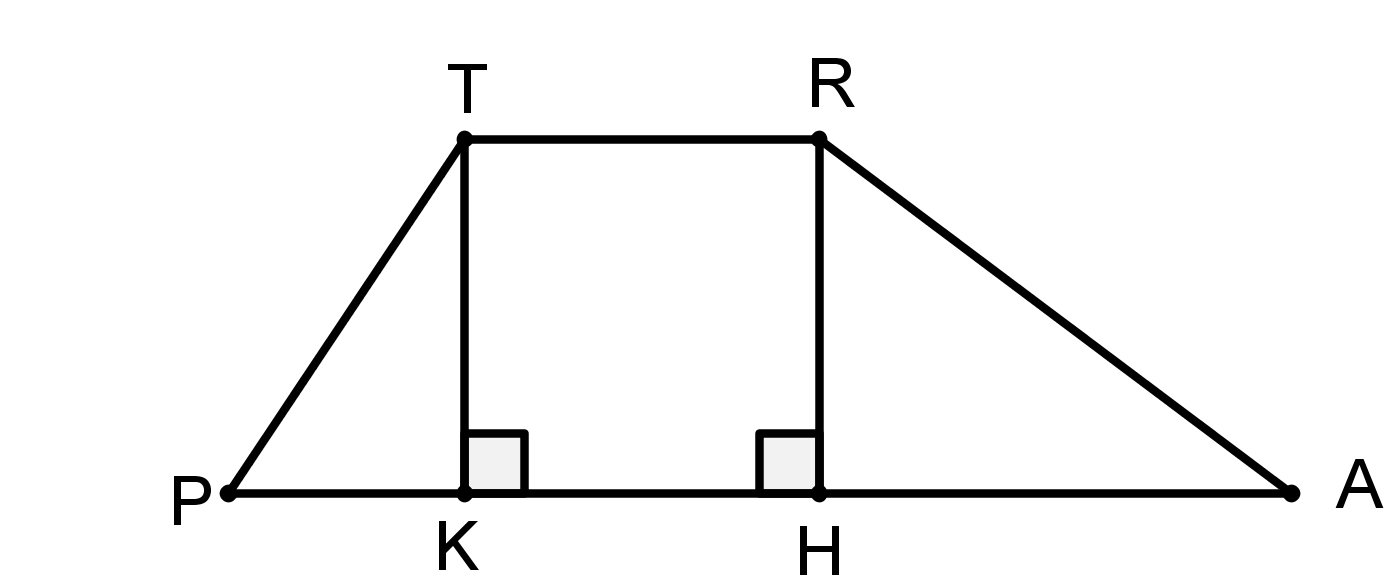
\includegraphics[width=6cm]{images/ex3.png}
\end{center}

\end{minipage}
&

\qquad \qquad \quad \qquad 
&
\begin{minipage}{8cm}
\ul{Exercice 4}: (\textit{3,5 points})


\begin{center}
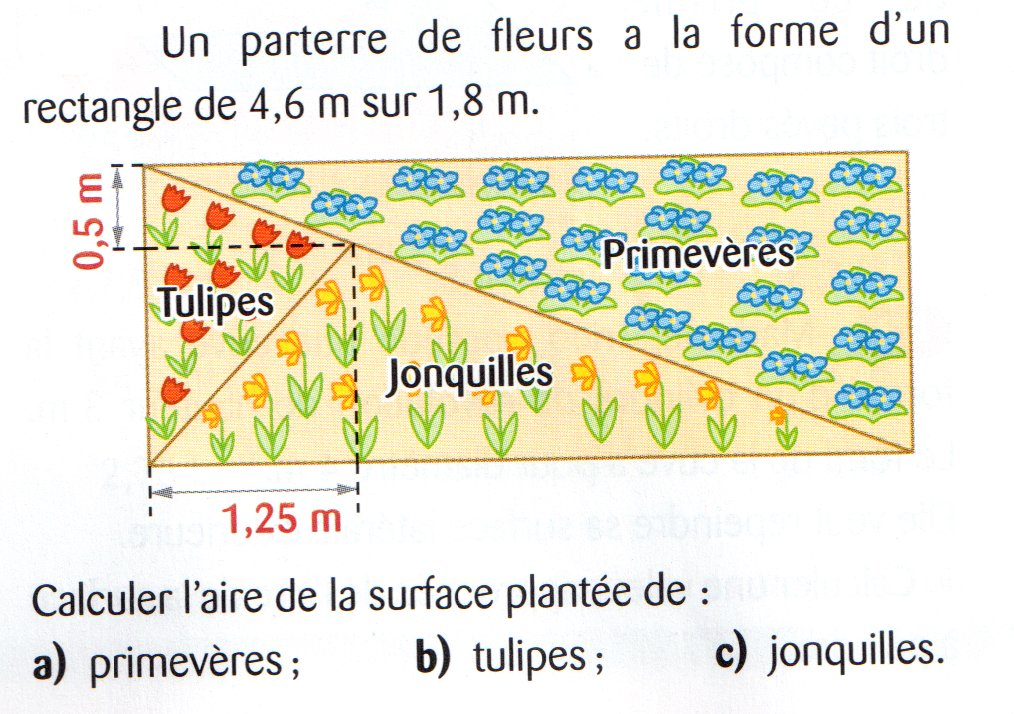
\includegraphics[width=8cm]{images/ex4.jpg}
\end{center}
Justifier toutes vos r�ponses. 
\end{minipage}
\end{tabular}





\medskip



\ul{Exercice 5}: (\textit{4 points})  

\enskip

\fbox{
\begin{minipage}{18cm}
\textbf{Cet exercice est un travail de
recherche. Les id�es et pistes de r�flexion seront prises en compte m�me si elles
n'aboutissent pas.}
\end{minipage}
}

 \enskip



Un navire qui se trouve au large de la floride (Etats-Unis) entend un S.O.S sur
les ondes de sa radio; ``Ici le capitaine de la \textit{Perle noire}, toutes
les boussoles de mon navire ne fonctionnent plus. Nous sommmes � �gale distance
d'Orlando, Hamilton et San Juan. Pouvez-vous venir nous aider?''

\enskip

\begin{tabular}{cc}
\begin{minipage}{10cm}



\begin{enumerate}
  \item A l'aide d'un papier calque (ou en reportant les mesures avec
  votre compas), reproduire le traingle des Bermudes trac� en rouge sur la
  carte.
  \item Donner la position de la \textit{Perle noire}. Expliquez votre d�marche.
\end{enumerate} 
\end{minipage}
&
\begin{minipage}{8cm}
 \qquad \qquad  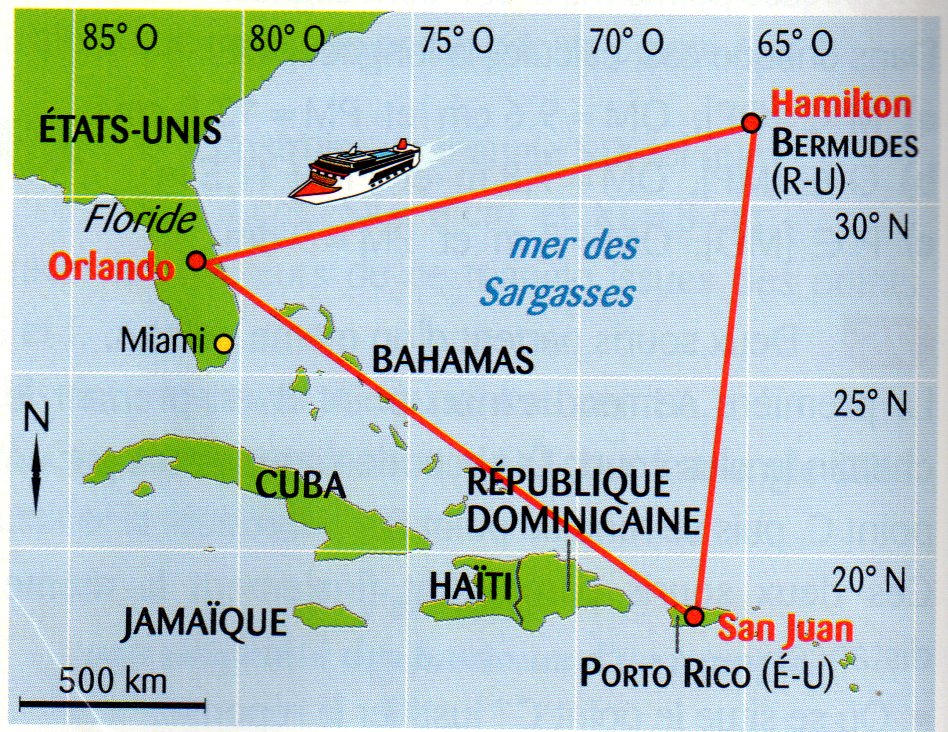
\includegraphics[width=6cm]{images/ex5.jpg}
\end{minipage}
\end{tabular}

\end{document}
